\section{Cross Section}
\label{sec:AN_CrossSection}

The cross section of $pp\rightarrow W\gamma \rightarrow l\nu\gamma$, where $l=\mu,e$, is measured as described in the beginning of Ch.~\ref{sec:AN_WgMeasStrategy} based on CMS data at $\sqrt{s}=$8~TeV in the phase space defined in  Ch.~\ref{sec:AN_WgMeas}. The measured cross section is compared to phase-space-corrected MCFM calculation at NLO which is referred as ``NLO theory''.  

The cross section of the simulated sample was computed with MCFM at NLO and is for the dedicated signal MC sample $\sigma_1=$553.92~pb. NNLO and higher corrections are expected to have an effect of \~20\%. The MC sample was generated with MadGraph, and the cross section in our selected phase space was computed as 

\begin{center}
$\sigma_2 = \sigma_1 \cdot \frac{N_2}{N_1}$, 
\end{center} 

\noindent{where  $N_2$ and $N_1$ are numbers of events falling into selected phase space and generated in the whole MC sample respectively. For the differential cross section, $N_2$ is number of events falling into specific $P_T^{\gamma}$ bin and to compute $\frac{d\sigma }{ dP_T^{\gamma}}$, we divide by the bin width.}

%\begin{center}
%\frac{{d\sigma }{ dP_T^{\gamma}}}, 
%\end{center} 
%\noindent{we divide by the bin width.} 

The total cross section is \\
$\sigma(W\gamma\rightarrow\mu\nu\gamma)=10949 \pm 91$ (stat.) $ \pm 2959$ (syst.) fb\\
for the muon channel, and \\
$\sigma(W\gamma\rightarrow\mu\nu\gamma)=9146 \pm 185$ (stat.) $ \pm 3981$ (syst.) fb\\
for the electron channel. the corresponding NLO theory values are 9139 and 9064~fb.

Tables~\ref{tab:sc_mc_vs_meas_MUON_WGamma}-\ref{tab:sc_mc_vs_meas_ELECTRON_WGamma} and Fig.~\ref{fig:CS_Wg} summarize the results of the differential cross section. The measured cross sections in different channels agree between each other as well as with the NLO theory cross section provided its accuracy.% The differential cross section can be used to derive limits on aTGC constants.

The measurement is systematically-dominated. For the muon channel, the most significant sources of the sytematic uncerntainty are sources associated with jets$\rightarrow\gamma$ background estimation. For the electron channel, uncerntainties on photon efficiency scale factors are more significant for certain bins. The relative systematic uncertainties on the total cross section are larger than those reported by the CMS measurement at $\sqrt{s}=$7~TeV~\cite{ref_7TeV_CMS}.

For validation of the measurement procedure, we measure the cross section of $Z\gamma$ and compare the result with the published CMS result for $Z\gamma$ at~8~TeV. We measure cross section in the muon and electron channels, in the same phase space as the published CMS measurement. 

$Z\gamma\rightarrow\mu\mu\gamma$ FSR and ISR datasets which are used to prepare real-$\gamma$ and fake-$\gamma$ templates for jets$\rightarrow\gamma$ background estimation largely overlap with nominally selected $Z\gamma$ dataset. Therefore, the measurement of $Z\gamma$ cross section in the muon channel is a closure check while the measurement of $Z\gamma$ cross section in the electron channel is a fully valid physics measurement. The results of our $Z\gamma$ measurement agree well with the published results (App.~\ref{sec:ZgCheck}).

The ongoing $W\gamma$ measurement based on~2015 and~2016 datasets has higher chances to discover a new physics if it presents because of higher energy of $\sqrt{s}=$13~TeV and higher statistical power of over~30~fb$^{-1}$. Although the largest uncertainties of the~8~TeV measurement are systematic uncertainties, many of them depend on amount of data in control samples, thus, the increased size of the data sample will help to reduce those uncerntainties. Higher collision energy allows to observe more signal events in high $P_T^{\gamma}$ ranges where the effect of potential aTGC is the largest. 

\begin{table}[h]
  \scriptsize
  \begin{center}
  \caption{Cross section and errors. $W\gamma$ at $\sqrt{s}=$8~TeV, muon channel. }
  \begin{tabular}{|c|c|c|}
    $P_T^{\gamma}$, & \multicolumn{2}{|c|} $d\sigma/dP_{T}$, [fb/GeV]  \\ 
    GeV & theory &    meas.       \\ \hline
%    total & 9139 & $10949 \pm 91 \pm 2959$ \\ \hline
%    10-15 & 1545 & $1765 \pm 33 \pm 278$ \\ \hline
    15-20 & 754 & $747 \pm 17 \pm 260$ \\ \hline
    20-25 & 382 & $419 \pm 10 \pm 142$ \\ \hline
    25-30 & 210 & $290 \pm 6 \pm 87$ \\ \hline
    30-35 & 129 & $175 \pm 5 \pm 78$ \\ \hline
    35-45 & 70 & $121 \pm 2 \pm 22$ \\ \hline
    45-55 & 36 & $34 \pm 1 \pm 23$ \\ \hline
    55-65 & 23 & $31 \pm 1 \pm 7$ \\ \hline
    65-75 & 13 & $16 \pm 1 \pm 7$ \\ \hline
    75-85 & 9 & $16 \pm 1 \pm 3$ \\ \hline
    85-95 & 6.3 & $9.8 \pm 0.5 \pm 2.4$ \\ \hline
    95-120 & 3.7 & $5.9 \pm 0.3 \pm 1.0$ \\ \hline
    120-500 & 0.27 & $0.41 \pm 0.01 \pm 0.10$ \\ \hline
  \end{tabular}
  \label{tab:sc_mc_vs_meas_MUON_WGamma}
  \end{center}
\end{table}

\begin{table}[h]
  \scriptsize
  \begin{center}
  \caption{Cross section and errors. $W\gamma$ at $\sqrt{s}=$8~TeV, electron channel.}
  \begin{tabular}{|c|c|c|}
    $P_T^{\gamma}$, & \multicolumn{2}{|c|} $d\sigma/dP_{T}$, [fb/GeV]  \\ 
    GeV & theory &    meas.       \\ \hline
%    total & 9064 & $9146 \pm 185 \pm 3981$ \\ \hline
%    10-15 & 1550 & $889 \pm 40 \pm 691$ \\ \hline
    15-20 & 749 & $440 \pm 35 \pm 396$ \\ \hline
    20-25 & 375 & $338 \pm 23 \pm 163$ \\ \hline
    25-30 & 210 & $298 \pm 16 \pm 107$ \\ \hline
    30-35 & 129 & $193 \pm 9 \pm 82$ \\ \hline
    35-45 & 71 & $103 \pm 3 \pm 29$ \\ \hline
    45-55 & 34 & $34 \pm 3 \pm 24$ \\ \hline
    55-65 & 22 & $31 \pm 2 \pm 18$ \\ \hline
    65-75 & 14 & $19 \pm 1 \pm 12$ \\ \hline
    75-85 & 9 & $12 \pm 1 \pm 8$ \\ \hline
    85-95 & 6.4 & $10.0 \pm 0.9 \pm 4.3$ \\ \hline
    95-120 & 3.6 & $4.9 \pm 0.4 \pm 2.5$ \\ \hline
    120-500 & 0.26 & $0.46 \pm 0.02 \pm 0.22$ \\ \hline
  \end{tabular}
  \label{tab:sc_mc_vs_meas_ELECTRON_WGamma}
  \end{center}
\end{table}
 
\begin{figure}[htb]
  \begin{center}
   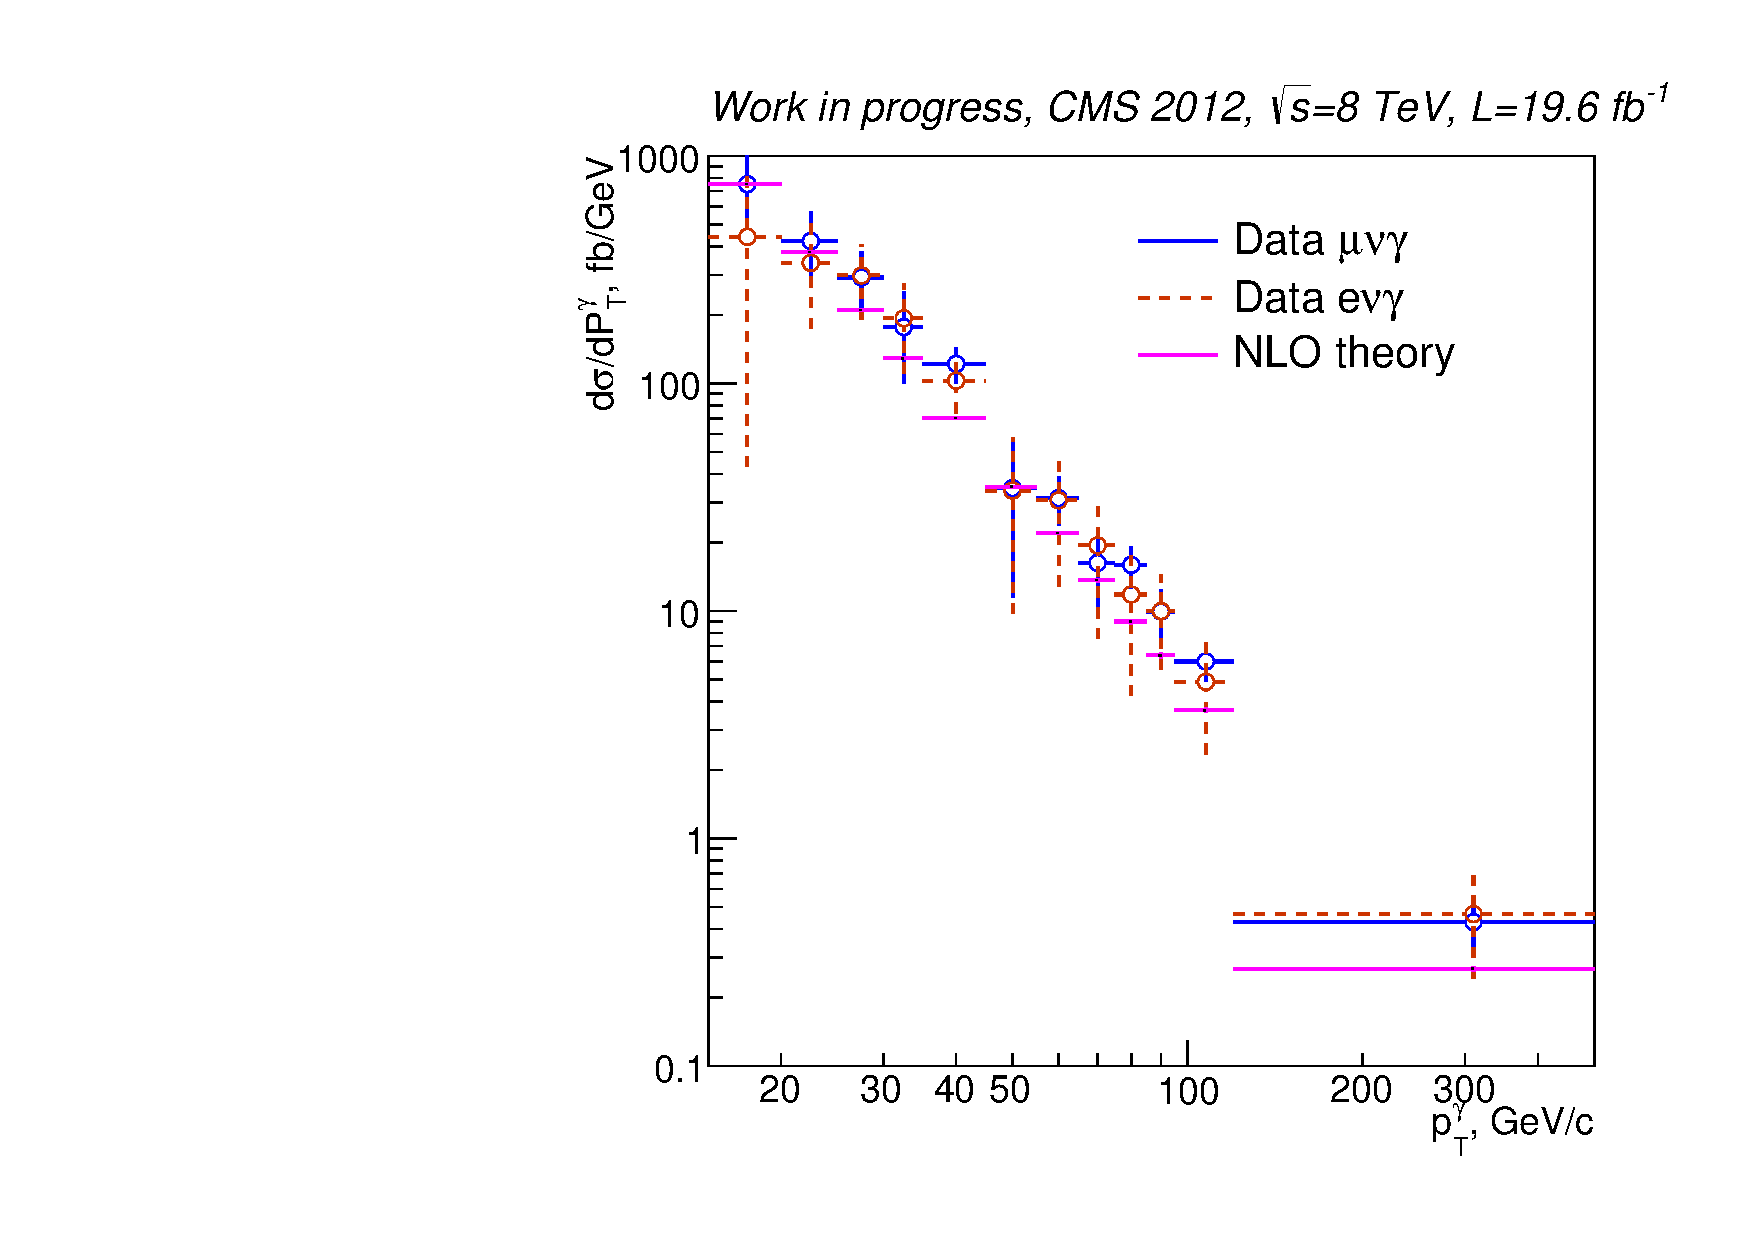
\includegraphics[width=0.5\textwidth]{../figs/figs_v11/ChannelsMERGED_WGamma/CrossSection/compareCSWGamma.pdf}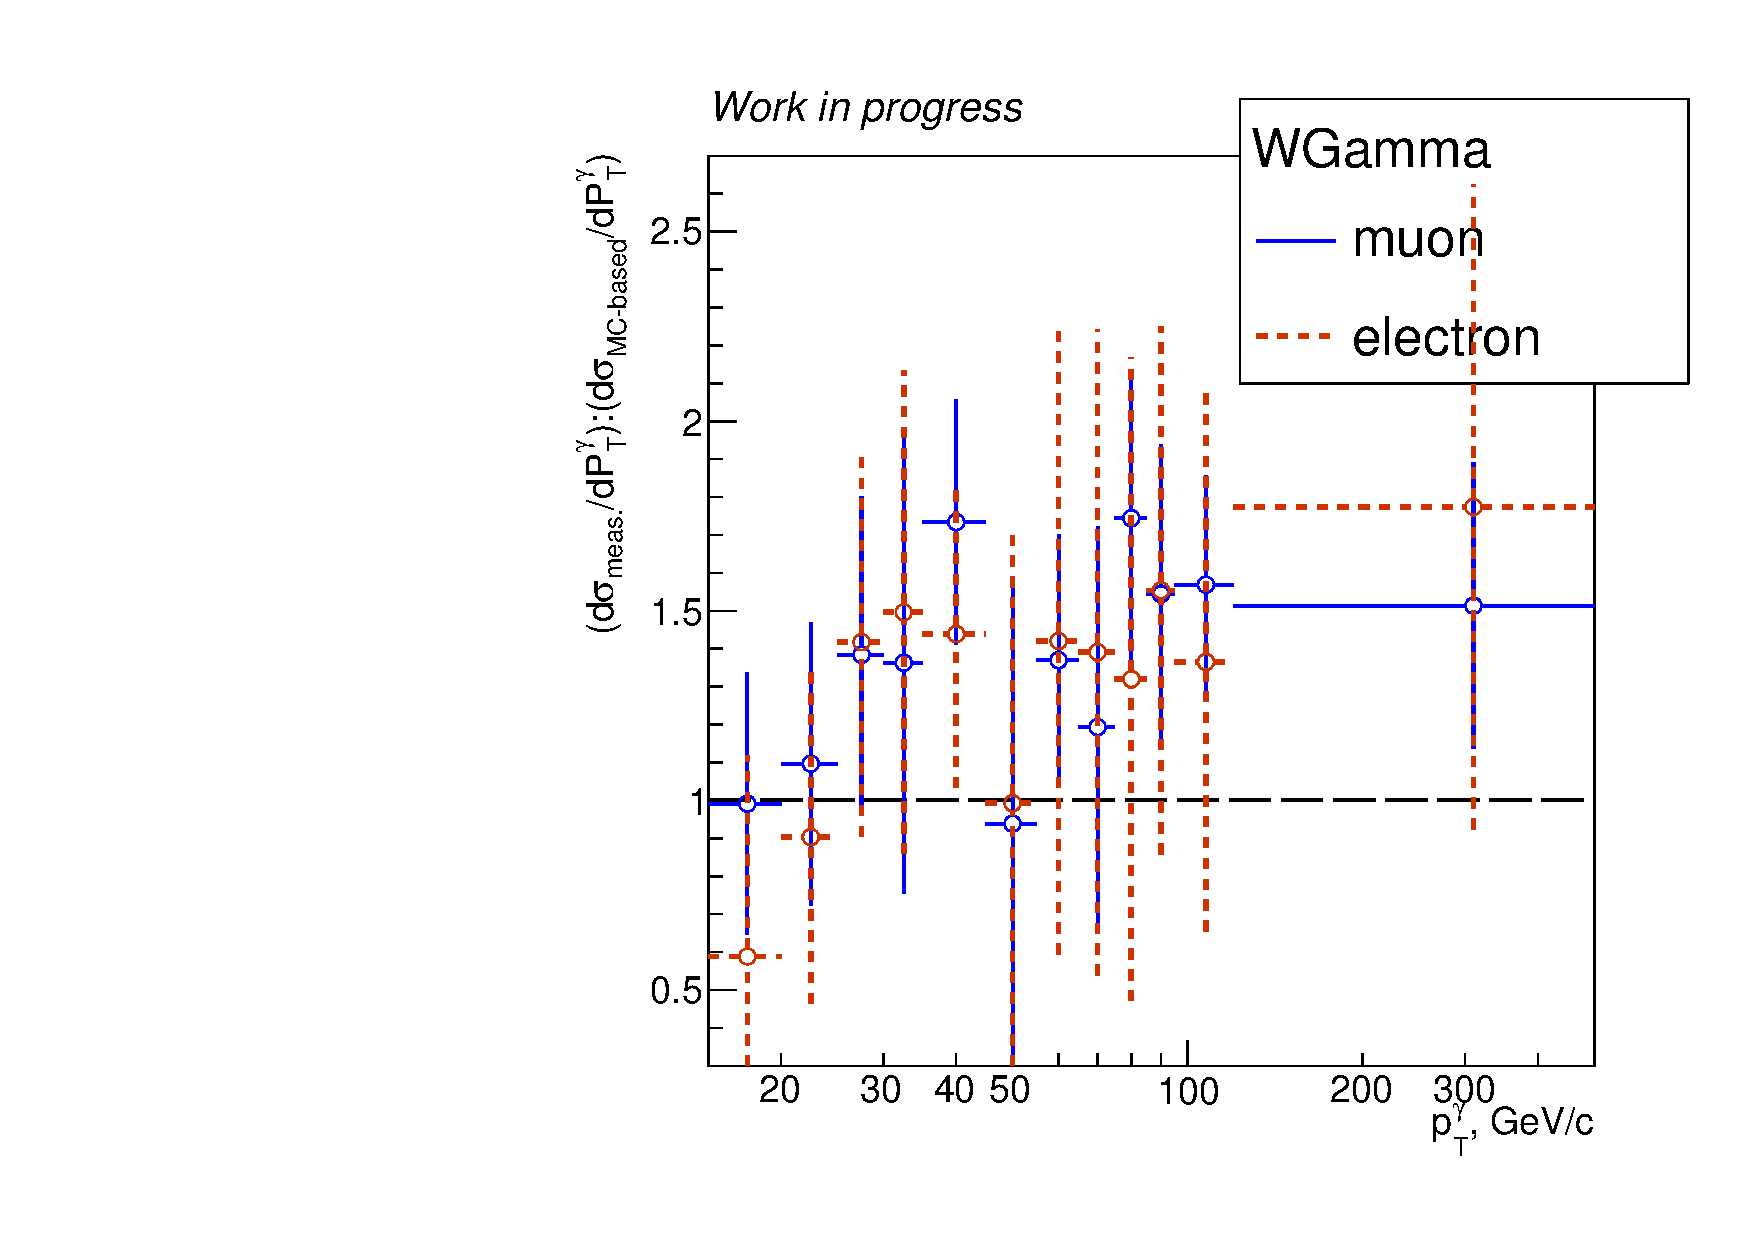
\includegraphics[width=0.5\textwidth]{../figs/figs_v11/ChannelsMERGED_WGamma/CrossSection/compareCSratioTheoryWGamma.pdf}
      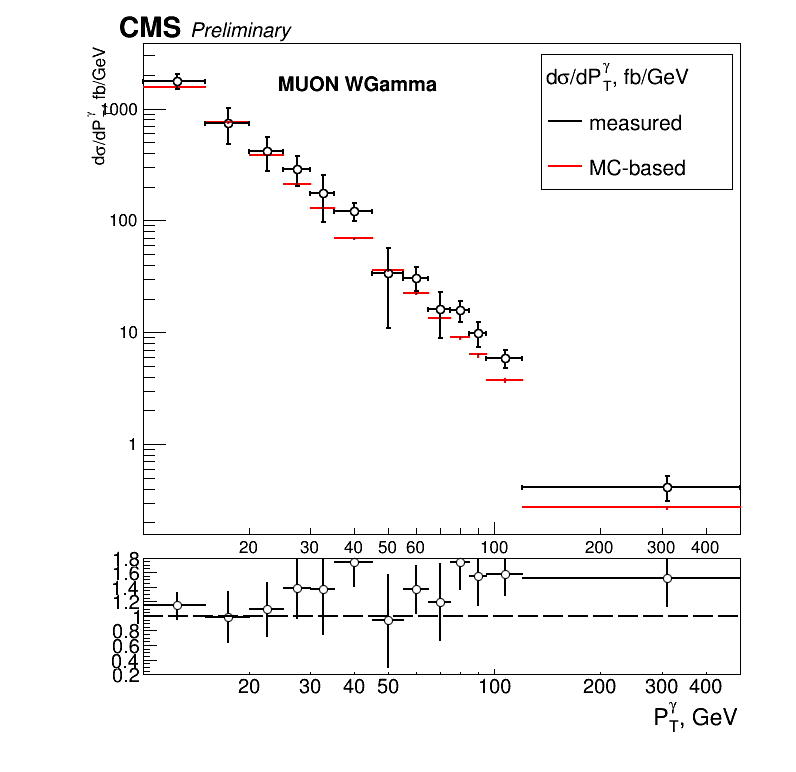
\includegraphics[width=0.48\textwidth]{../figs/figs_v11/MUON_WGamma/CrossSection/c_CS_MUON_WGamma_UNblind.png} 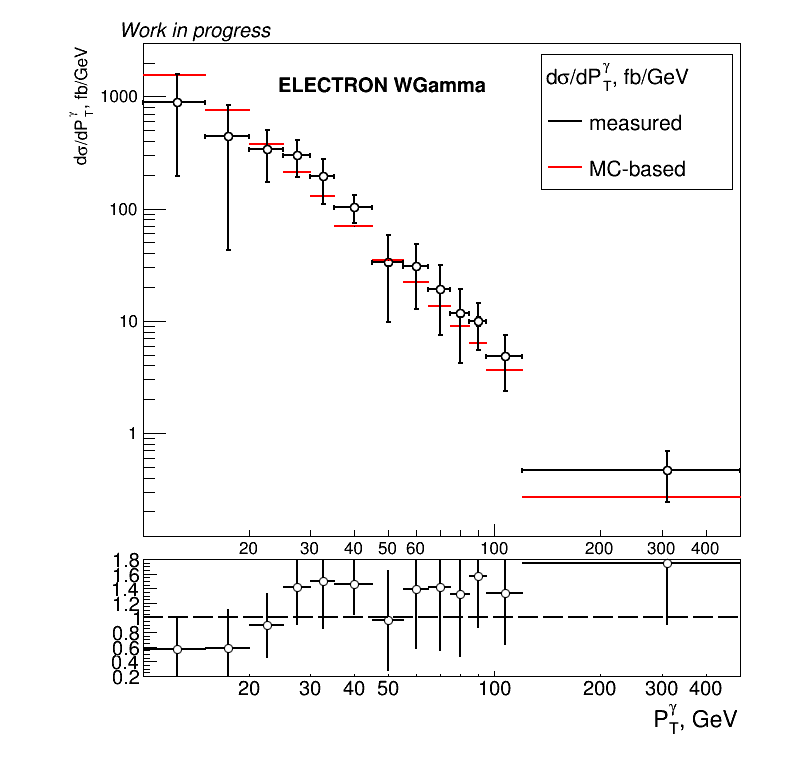
\includegraphics[width=0.48\textwidth]{../figs/figs_v11/ELECTRON_WGamma/CrossSection/c_CS_ELECTRON_WGamma_UNblind.png}
  \caption{$W\gamma$ differential cross section. Top, left: the $W\gamma$ differential cross section; top, right: the ratio of measured over the MC-based $W\gamma$ differntial cross section. Bottom:  the $W\gamma$ measured differential cross section overlaid with the MC-based cross section in the muon channel (left) and in the electron channel (right).}
  \label{fig:CS_Wg}
 \end{center}
\end{figure}



